\documentclass[../manuscript.tex]{subfiles}
\section{Заключение. План дальнейших исследований}

В данной работе представлен новый подход к решению двух важных задач вычислительной онкологии: \begin{itemize}
	\item Восстановления клональной структуры опухоли;
	\item Предсказания аллель-специфических структурных вариаций.
\end{itemize}
Изначально была и третья, главная задача — перенос клональной структуры с ДНК-образца на существенно более дешёвые РНК-образцы. Достичь в ней успеха не позволила разреженность РНК-данных. В связи с этим было решено сосредоточиться на ДНК-данных и решении первых двух задач. 

Метод получил временное название XClone и представляет собой графическую байесовскую модель опухоли. XClone опирается на два важных типа биологических сигналов в данных секвенирования: 
\begin{itemize}
	\item BAF — аллельный дисбаланс, насколько чаще прочтения выравниваются на материнский аллель;
	\item RDR — амплификация доли прочтений, насколко чаще прочтения выравниваются на участок генома чем это предсказывает вероятностная модель секвенирования.
\end{itemize}
Разработанные алгоритмы предобработки данных показали, что оба этих сигнала можно надёжно извлекать из данных ДНК-секвенирования одиночных клеток, несмотря на их разреженность. В случае BAF-сигнала это долгое время считалось нерешённой задачей. Был предложен метод аггрегирования гетерозиготных ОНП с сохранением тренда аллельных частот на основе ЕМ-алгоритма, который показывает хорошие результаты на реальных данных. Этот метод представляет отдельный интерес, т.к. сам по себе имеет научную новизну.

В данной работе представлены две последовательные версии этого алгоритма, XClone-V1 и XClone-V2. Их различия резюмирует следующая таблица:

\begin{table}[H]
	\centering
	\begin{tabular}{|p{4cm}|p{5cm}|p{5cm}|}
		\hline
		\textbf{Версия} & \textbf{XClone-V1} & \textbf{XClone-V2}\\ 
		\hline
		\textbf{Главная задача} & Перенос клональной структуры ДНК-образца на РНК-образец & Поиск аллель-зависимых структурных вариаций и восстановление по ним клональной структуры ДНК-образца \\
		\hline
		\textbf{Метод вывода} & Семплирование по Гиббсу & Вариационный байесовский вывод\\
		\hline
		\textbf{Реализация} & Pure Python + numpy, scipy, numba & Tensorflow 2.0\\
		\hline
		\textbf{Поддержка} GPU & Нет & Да\\
		\hline
	\end{tabular}
\end{table}

Оба метода показали хорошее качество на синтетических данных. В силу разреженности реальных РНК-данных, от XClone-V1 пришлось отказаться, в связи с чем большая часть результатов, представленных в данной работе, получена уже с помощью XClone-V2. Было продемонстрировано, что XClone-V2 может с высокой долей достоверности воспроизвести аллель-специфические структурные вариации по данным, извечённым из реальной опухоли — медуллобластомы, детской опухоли мозга — на коммерческой платформе 10X Genomics, основных производителей оборудования для секвенирования одиночных клеток. 

На данный момент, у XClone-V2 есть только один непосредственный конкурент — алгоритм CHISEL\cite{ChiselBiorxiv}, опубликованный в ноябре 2019 года учёнными из лаборатории Бена Рафаэля, Принстон. Результаты CHISEL и XClone-V2 согласуются, при этом XClone-V2 работает гораздо быстрее, порядка 10 минут против нескольких часов CHISEL на CPU, а на GPU ещё в несколько раз быстрее ( CHISEL не поддерживает GPU вовсе). Кроме того, вариационный байесовский вывод в XClone-V2 происходит автоматически, т.к. его удалось выразить в синтаксисе Tensorflow.Probability. Благодаря этому в XClone-V2, в отличие от CHISEL, можно легко совершенствовать статистическую модель и добавлять в неё поддержку новых модальностей (scRNA-seq, scATAC-seq, соматические мутации, митохондриальная ДНК), чтобы использовать все имеющиеся под рукой данные для уточнения диагноза. Такой подход позволяет в перспективе разработать линейку специализированных методов под разные нужды учёных и врачей. 

Экспериментально были выяснены и недостатки модели XClone-V2, подробно описанные в конце главы "Материалы и методы". Их анализ позволил разработать проект новой, улучшенной версии алгоритма — XClone-V3, в которой RDR-составляющая заменена с мультиномиальной модели, которую трудно оптимизировать и в которой неявно создаются лишние зависимости между признаками, на модели, симметричной BAF-модулю и использующей отрицательное биномиальное распределение для моделирования числа прочтений в сегментах генома опухолевых клеток. Это стандартный подход в моделировании данных ДНК-секвенирования одиночных клеток, и авторы убеждены, что он будет давать лучшие результаты.

\begin{figure}[H]
	\centering
	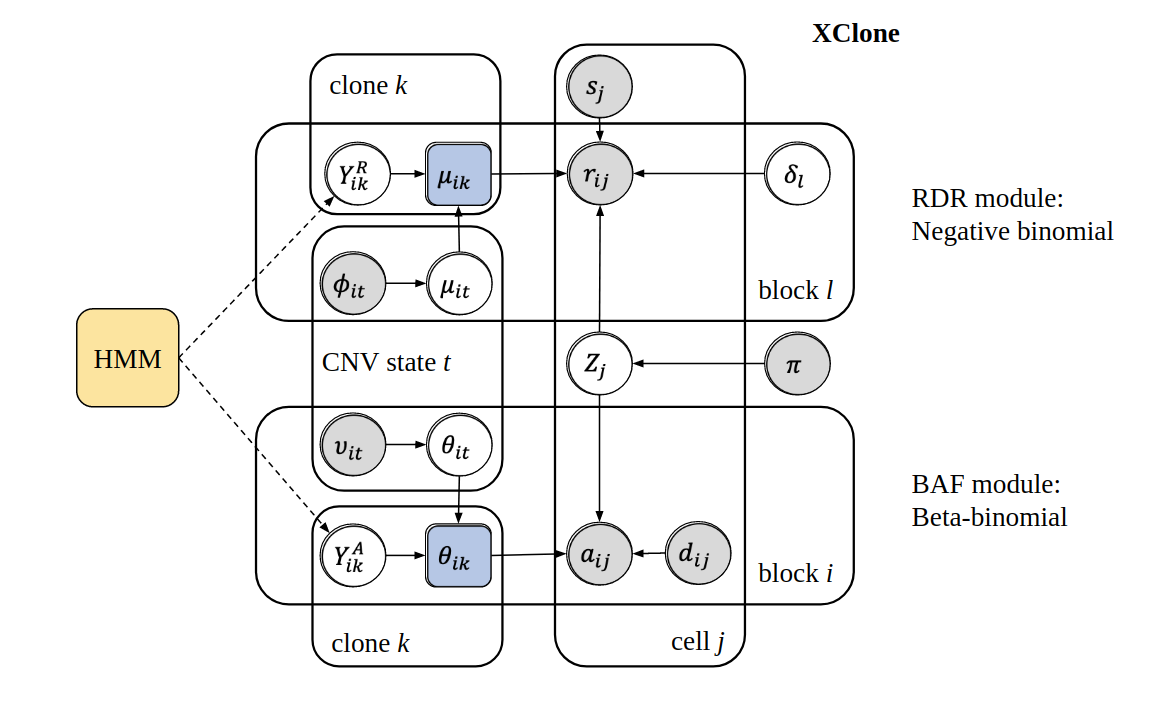
\includegraphics[keepaspectratio=true,scale=0.4]{images/xclone_v3.png}
	\caption{Третья версия алгоритма XClone в plate notation.}
\end{figure}

Кроме того, продвижения в задаче определения структурных вариаций по данным scRNA-seq, а именно алгоритм InferCNV, вдохновили авторов вернуться к решению первоначальной задачи — переносу клональной структуры с ДНК-образца на РНК-образцы, — в этот раз на основе преобразованных RDR-сигналов, аналогичных тем, что используются в методе InferCNV. Увы, имеющиеся данные, в силу однородности опухоли, ограничивают дальнейшую разработку метода. В связи с этим данный момент идут перегоровы с лабораторией Кристины Кёртис, Стэнфорд, с целью валидации алгоритма XClone-V3 на образцах опухоли желудка с значительно более богатой клональной структурой (порядка 10 клональных линий) и дальнейшей коллаборации. Если XClone-V3 покажет хорошие результаты, это будет первый алгоритм предсказания аллель-специфических структурных вариаций по данным scRNA-seq, что позволит опубликовать метод в высокоимпактном журнале. 